\documentclass{standalone}
\usepackage{tikz}
\usepackage{ctex,siunitx}
\setCJKmainfont{Noto Serif CJK SC}
\usepackage{tkz-euclide}
\usepackage{amsmath}
\usetikzlibrary{patterns, calc,3d}
\usetikzlibrary {decorations.pathmorphing,decorations.pathreplacing,decorations.shapes}
\begin{document}
\small
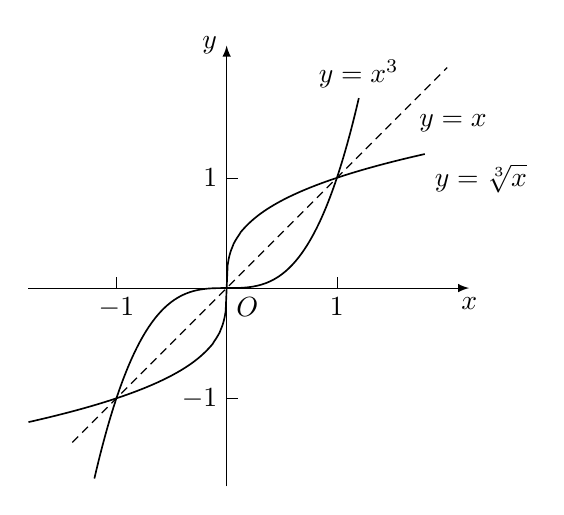
\begin{tikzpicture}[>=latex,scale=1.4]
  \draw[->](-1.8,0)--(2.2,0)node[below]{$x$};
  \draw[->](0,-1.8)--(0,2.2)node[left]{$y$};
  \node at (0,0)[below right]{$O$};
  \draw[densely dashed](-1.4,-1.4)--(2,2)node[pos=0.9,below right]{$y=x$};
  \draw[semithick,samples=200,domain=-1.2:1.2]plot(\x,{pow(\x,3)})node[above]{$y=x^3$};
  \draw[semithick,samples=200,domain=0:1.8]plot(\x,{pow(\x,1/3)})node[below right]{$y=\sqrt[3]{x}$};
  \draw[semithick,samples=200,domain=0:-1.8]plot(\x,{-pow(-\x,1/3)});
  \foreach \x in {1,-1} 
    { 
      \draw[very thin] (\x,0)node[below]{$\x$}--++(0,0.1); 
      \draw[very thin] (0,\x)node[left]{$\x$}--++(0.1,0); 
    }
\end{tikzpicture}
\end{document}